% Figure 1
\begin{figure}[t]
  \centering
  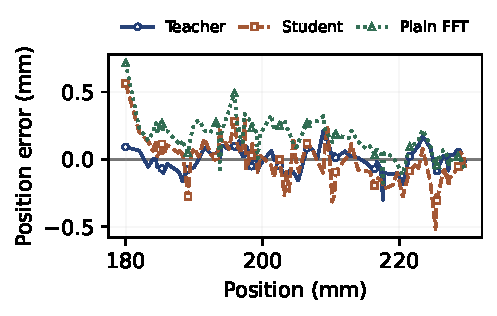
\includegraphics[width=0.95\columnwidth]{paper_outputs/fig01_position_error_curves_singlecol.pdf}
  \caption{Position error curves of Teacher, Student, and Plain FFT across the validation positions. All methods are evaluated on the same file set and mapped with a shared calibration model.}
  \label{fig:pos_err}
\end{figure}

% Figure 2
\begin{figure}[t]
  \centering
  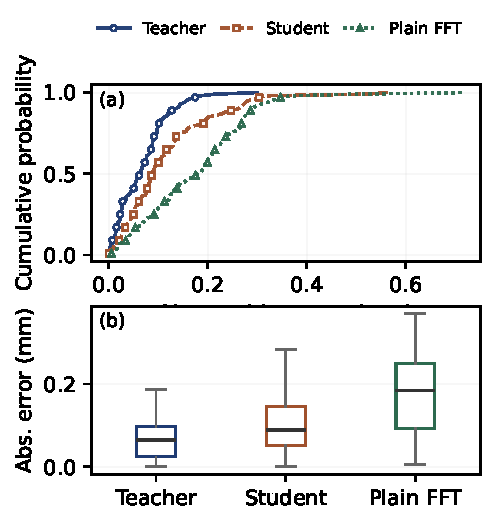
\includegraphics[width=0.95\columnwidth]{paper_outputs/fig02_error_distribution_singlecol.pdf}
  \caption{Error distribution comparison for Teacher, Student, and Plain FFT: (a) empirical CDF of absolute position errors; (b) boxplot of absolute position errors.}
  \label{fig:err_dist}
\end{figure}

% Figure 3
\begin{figure}[t]
  \centering
  \includegraphics[width=0.95\columnwidth]{paper_outputs/fig03_accuracy_latency_tradeoff_singlecol.pdf}
  \caption{Accuracy--efficiency tradeoff for Teacher, Student, and Plain FFT. The x-axis shows per-file latency (log scale) and the y-axis shows position MAE.}
  \label{fig:tradeoff}
\end{figure}

% Figure 4
\begin{figure}[t]
  \centering
  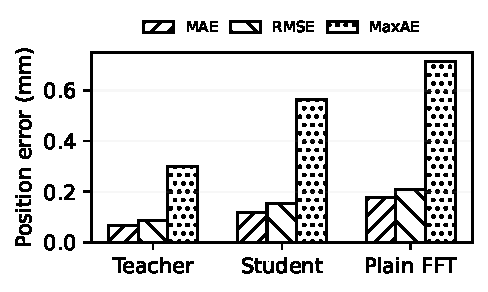
\includegraphics[width=0.95\columnwidth]{paper_outputs/fig04_summary_bars_singlecol.pdf}
  \caption{Grouped comparison of MAE, RMSE, and MaxAE for Teacher, Student, and Plain FFT.}
  \label{fig:summary_bars}
\end{figure}

% Tables
\begin{table}[t]
\centering
\caption{Main quantitative comparison of Teacher, Student, and Plain FFT on the same validation files.}
\label{tab:main_quant}
\begin{tabular}{lccccc}
\hline
Method & Width MAE (pixel) & Pos. MAE (mm) & Pos. RMSE (mm) & Pos. MaxAE (mm) & Latency (ms) \\ 
\hline
Teacher & 0.0000 & 0.0678 & 0.0858 & 0.2999 & NA \\
Student & 0.0000 & 0.1166 & 0.1530 & 0.5641 & NA \\
Plain FFT & 0.0397 & 0.1761 & 0.2088 & 0.7149 & 3.166 \\
\hline
\end{tabular}
\end{table}

\begin{table}[t]
\centering
\caption{Compact speed--accuracy summary.}
\label{tab:compact_speed}
\begin{tabular}{lccc}
\hline
Method & Pos. MAE (mm) & Speedup vs Teacher & Note \\ 
\hline
Teacher & 0.0678 & NA & Reference \\
Student & 0.1166 & NA & Near-teacher \\
Plain FFT & 0.1761 & NA & Classical baseline \\
\hline
\end{tabular}
\end{table}

